\let\negmedspace\undefined
\let\negthickspace\undefined
\documentclass[journal,12pt,twocolumn]{IEEEtran}
\usepackage{cite}
\usepackage{amsmath,amssymb,amsfonts,amsthm}
\usepackage{algorithmic}
\usepackage{graphicx}
\usepackage{textcomp}
\usepackage{xcolor}
\usepackage{txfonts}
\usepackage{listings}
\usepackage{enumitem}
\usepackage{mathtools}
\usepackage{gensymb}
\usepackage{comment}
\usepackage[breaklinks=true]{hyperref}
\usepackage{tkz-euclide} 
\usepackage{listings}
\usepackage{gvv}  
\usepackage{tikz}
\usepackage{circuitikz} 
\usepackage{caption}
\def\inputGnumericTable{}              
\usepackage[latin1]{inputenc}          
\usepackage{color}                    
\usepackage{array}                     
\usepackage{longtable}                 
\usepackage{calc}                     \usepackage{multirow}                  
\usepackage{hhline}                    
\usepackage{ifthen}                    
\usepackage{lscape}
\usepackage{amsmath}
\newtheorem{theorem}{Theorem}[section]
\newtheorem{problem}{Problem}
\newtheorem{proposition}{Proposition}[section]
\newtheorem{lemma}{Lemma}[section]
\newtheorem{corollary}[theorem]{Corollary}
\newtheorem{example}{Example}[section]
\newtheorem{definition}[problem]{Definition}
\newcommand{\BEQA}{\begin{eqnarray}}
\newcommand{\EEQA}{\end{eqnarray}}
\newcommand{\define}{\stackrel{\triangle}{=}}
\theoremstyle{remark}
\newtheorem{rem}{Remark}

%\bibliographystyle{ieeetr}
\begin{document}
%

\bibliographystyle{IEEEtran}




\title{
%	\logo{
G.A.T.E.

\large{EE1205 : Signals and Systems}

Indian Institute of Technology Hyderabad
%	}
}
\author{Chirag Garg

(EE23BTECH11206)
}	





\maketitle

\newpage



\bigskip

\renewcommand{\thefigure}{\theenumi}
\renewcommand{\thetable}{\theenumi}


\section{Question E.C.(45)}
\vspace{0.5cm}



\textbf{Question:} Let a frequency modulated (FM) signal : $ x(t) = A \cos(\omega_c t + k_f \int_{-\infty}^{t} m(\lambda) d\lambda)$ , where $ m(t) $is a message signal of bandwidth $ W $. It is passed through a non-linear system with output $y(t) = 2x(t) + 5(x(t))^2 $.
Let $B_T $denote the FM bandwidth. The minimum value of $ \omega_c $ required to recover $ x(t) $ from $ y(t) $ is:\\
\begin{enumerate}[label = (\Alph*)]
\item $B_T + W$ \\
\item $\dfrac{3}{2} B_T$ \\
\item $2B_T + W$ \\
\item $\dfrac{5}{2} B_T$ \\
\end{enumerate}
%\section{Solution} 
\textbf{Solution: }
Let $k_f \int_{-\infty}^{t} m(\lambda) d\lambda = \phi $
\begin{align}
 x(t) &= A \cos(\omega_c t + \phi) \\
 y(t) &= 2x(t) + 5(x(t))^2 \\
 &= 2A \cos(\omega_c t + \phi) + 5A^{2}\cos^{2}(\omega_c t +  \phi  ) \\
 &= 2A \cos(\omega_c t +  \phi ) + \dfrac{5}{2}A^{2}[\cos(2\omega_c t +  2\phi ) + 1]
 \end{align}
\begin{figure}[h!]
  \centering
  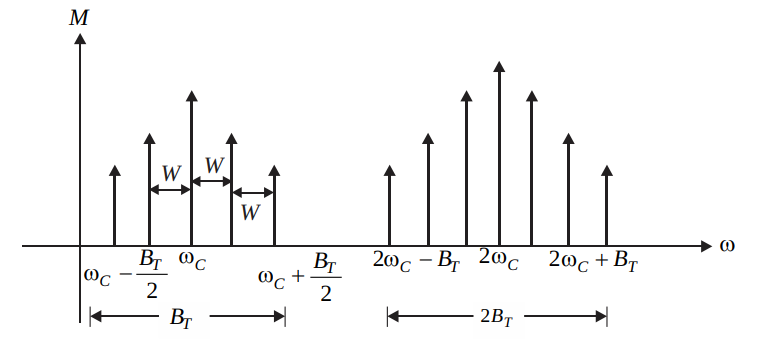
\includegraphics[width=0.5\textwidth]{figures/cggate.png} 
 \label{cggatefig1}
 \caption*{Fig 1: Plot of M(Modulation Frequency) vs $\omega$  }
\end{figure}
\\From garph ,to recover $x(t)$ from $y(t)$
\begin{align}
2\omega_c - B_T > \omega_c + \dfrac{B_T}{2} \\
\omega_c > \dfrac{3B_T}{2} \\
\therefore(\omega_c)_{min} = \dfrac{3}{2}B_T
\end{align}
Hence the correct option is $(b)$
\end{document}